\section{Propuesta}

El diseño ideal para contribuir con la solución del problema es: una herramienta
que contenga el setup de Jif para Android, e integre un clasificador de
sources y sinks. De manera que, la herramienta evalúe flujos de información en
aplicativos Android, para verificar el cumplimiento de las políticas de
seguridad que el desarrollador define en el código, mediante el sistema de
anotaciones de Jif.\newline
Sin embargo, para efectos del presente trabajo se limita el Setup de Jif,
partiendo de una política de seguridad específica. Así, el diseño se centra en
soportar un conjunto reducido de clases de la API de Android(Anotaciones a la
API), y en incluir un conjunto específico de sources y sinks; de acuerdo a una
política de seguridad establecida. Ese conjunto de sources y sinks, se toma del
listado de sources y sinks proveído por SuSi \ref{sec:susi}.\newline 
Adicionalmente, para aspectos de evaluación, se incluye el diseño de un
anotador que automatiza la anotación requerida por el desarrollador.
De modo que, acorde a la política de seguridad establecida, se genere la
versión anotada del aplicativo a analizar.\newline
La figura \ref{fig:desingReal} muestra el esquema del diseño, allí los componentes
principales son el \emph{generador de anotaciones} y la \emph{herramienta de
análisis estático}.\newline 
Para retornar la versión Jif del aplicativo, el \emph{generador de anotaciones}
parte del código fuente de la aplicación Android a analizar, la política de
seguridad a evaluar, y los sources y sinks requeridos para verificar tal
política.\newline 
Luego esa versión Jif del aplicativo se debe pasar como entrada a la herramienta
de análisis estático, la cual retorna el análisis de flujo de
información.\newline 
La \emph{herramienta de análisis estático}, está integrada
por el compilador de Jif(verificador de políticas) y las anotaciones a la API de Android. Con
anotaciones a la API se hace referencia a clases de la API android que deben ser
reconocidas por el compilador de Jif, para verificar el cumplimiento de la
política de seguridad establecida. Cabe anotar que, tal reconocimiento no
implica modificaciones al compilador de Jif.

\begin{figure}[t!]
	\begin{center} 
	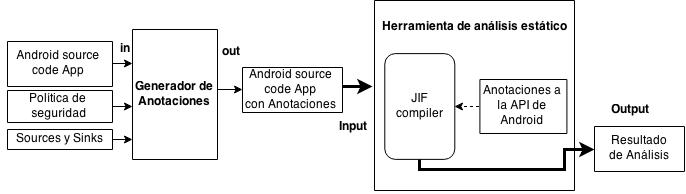
\includegraphics[width=8.5cm]{desing3Real-2-2.jpg} 
	\end{center}
	\caption{Diseño herramienta de análisis estático. 
	El generador de anotaciones retorna la versión anotada del aplicativo a
	analizar, partiendo del código fuente del aplicativo Android, la
	política de seguridad a evaluar, más los sources y sinks requeridos para
	verificar la política. La herramienta de análisis estático está integrada por
	el compilador de Jif, más anotaciones a la API de Android. Esta recibe el
	aplicativo Android debidamente anotado y retorna el análisis de flujo de
	información.}
	\label{fig:desingReal}
\end{figure}

Siguiendo el esquema de diseño anteriormente descrito: primero, se define la
política de seguridad a evaluar \ref{subsection:politica}; segundo, se toman a
consideración elementos influyentes para verificar el cumplimiento de la
política mediante Jif \ref{subsec:consVerPol}; y tercero, teniendo en cuenta
\ref{subsection:politica} y \ref{subsec:consVerPol}, se definen los lineamientos
de anotación \ref{sec:lineamientos}. Tales lineamientos establecen el esquema
para anotaciones a la API Android y anotaciones a los aplicativos a
analizar(lineamientos del anotador).

\subsection{Definición de la política de seguridad}
% \textit{Definición de la política de seguridad}:
Detectar si una aplicación Android(perteneciente al conjunto evaluable) presenta
flujos de información entre, información con nivel de seguridad alto e
información con nivel de seguridad bajo.\newline
Detectando fugas de información catalogada con nivel de seguridad alto, vía:
canales creados durante el control de flujo del programa(flujos implícitos),
mensajes de texto y mensajes de Log.\newline 
\textit{Información considerada con nivel de seguridad alto}: sources
caracterizados por dar a conocer información del usuario, considerada como
privada o sensible. Los métodos que integran el conjunto de sources son:
getDeviceId, getSimSerialNumber, findViewById, getLatitude, getLongitude y
getSubscriberId. Adicional a estos métodos, se incluye el tipo de dato EditText,
si y sólo si, el campo UI al que referencia corresponde a un campo tipo
textPassword, campos destinados a almacenar contraseñas.\newline 
Este conjunto de sources es tomado del listado proveído por el clasificador SuSi \ref{sec:susi}.


\subsection{Lineamientos de anotación}
Los lineamientos de anotación definen los elementos básicos de anotación
\ref{subsec:elements}, anotaciones necesarias para la API de Android
\ref{subsec:api} y anotaciones en los aplicativos a analizar \ref{subsec:anotador}.

\subsubsection{Elementos básicos de anotación}
Para anotar la información con su respectivo nivel de seguridad alto o bajo, de
modo que, partiendo de tales anotaciones se evalúe la existencia de flujos de
información entre información con nivel de seguridad alto e información con
nivel de seguridad bajo, se define una autoridad para los programas y los labels
de seguridad.\newline 

Principal \emph{Alice}\newline
haciendo uso de los principals ya definidos en Jif, se establece al principal
\emph{Alice} como la autoridad máxima. Este principal tendrá todo el poder para
actuar sobre aspectos de los programas.

Label de seguridad \emph{\{Alice:\}}\newline
este label indica que la información tiene nivel seguridad alto, es decir, que
se trata de información sensible o privada.\\
Variables con nivel de seguridad alto deben ser anotadas con tal label de
seguridad, porque esté específica que sólo el dueño de la información(Alice)
puede acceder a la misma. 

Label de seguridad \emph{\{\}}\newline
este label indica que la información tiene nivel de seguridad bajo, es decir,
información de conocimiento público.


\subsubsection{Incluir Resultados de evaluación XXX}





















